\chapter{Implementierung}
\label{cha:implementierung}

In diesem Kapitel wird die Auswahl der für die Umsetzung benötigten Komponenten beschrieben und deren Kommunikation und Schnittstellen geklärt. Anschließend werden Anmerkungen zur Implementierung gegeben und der Workflow anhand von Beispielen verdeutlicht. Den Kern des Kapitels bilden die drei Hauptkomponenten bestehend aus \textit{Android Applikation}, \textit{Dialogflow Agent} und \textit{Node.js Webservice}.

\section{Auswahl der Komponenten}
\label{sec:auswahl-komponenten}

In diesem Kapitel werden die verwendeten Plattformen und Komponenten beschrieben. Als Vorlage dient dabei der in \ref{subsec:cui-chatbot} vorgestellte Aufbau eines Chatbots. Einige der Komponenten sind dabei von Beginn an festgelegt, bei anderen bedarf es einer technischen Einordnung oder Entscheidungsfindung. Abbildung \ref{fig:Komponenten-v1} zeigt die drei Hauptkomponenten und die Interaktion des Users.
\newline

\begin{figure}[htb]
    \centering
    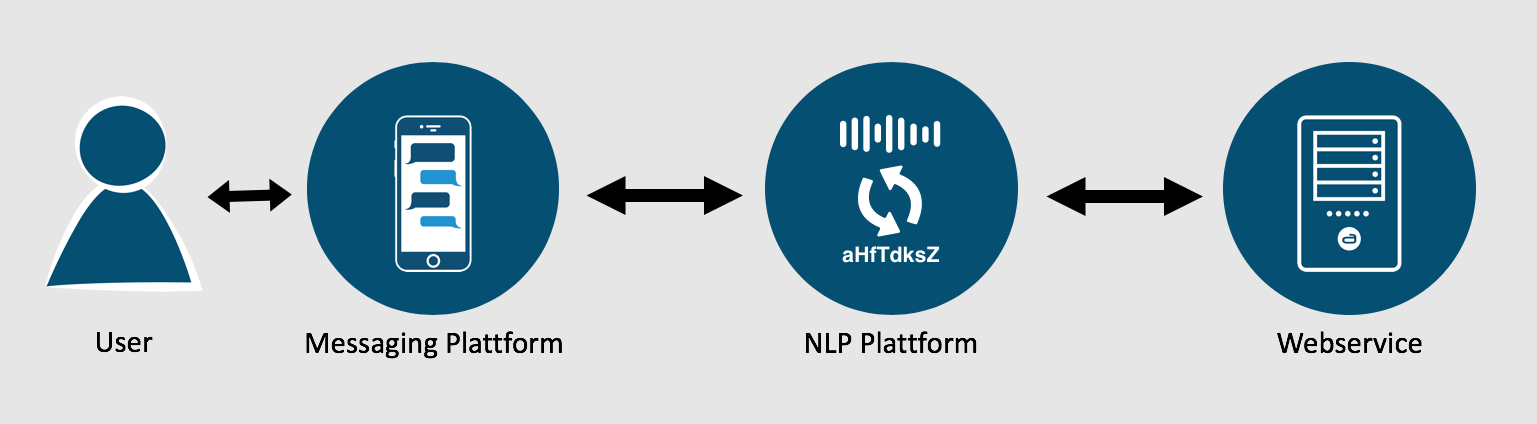
\includegraphics[width=0.9\textwidth]{bilder/Komponenten-v1.png}
    \caption{Übersicht der drei Hauptkomponenten}
    \label{fig:Komponenten-v1}
\end{figure}

\subsection{Frontend}
\label{subsec:frontend}

Zu Beginn jeder Interaktion mit einem Chatbot steht ein Frontend oder, wie in \ref{subsec:cui-chatbot} bezeichnet, eine Messaging Platform. Diese stellt gewissermaßen das Interface dar, über das der User seine Nachrichten eingeben und abschicken kann. 

Wie bereits eingangs erwähnt, gibt es einige Nachrichtenplattformen, in denen Chatbots entwickelt und integriert werden können. Häufig verwendet werden hierbei der Facebook Messenger, WeChat oder Slack. Teilweise bieten diese Plattformen bereits die Möglichkeit zur Darstellung und Integration von \ac{UI}-Elementen in Form von Buttons oder Auswahllisten. Die Vorgehensweise und Umsetzung ist dabei allerdings gleichermaßen einfach wie begrenzt. Während es relativ unkompliziert möglich ist, Antwortmöglichkeiten auf die Frage eines Chatbots via Popup-Buttons zu visualisieren, sind komplexere oder modifizierte \ac{UI}-Elemente nur schwierig bis gar nicht \mbox{umsetzbar}. 

Nachdem die \adorsys \, den Google-Kalender nutzt gibt es von Beginn an den Wunsch bzw. die Idee, dass die Nutzer des Chatbots sich mit dem gewöhnlichen Firmenaccount und der Endung \textit{@adorsys.de} anmelden und authentifizieren können. Die Integration des Firmenkontos in eine andere Nachrichtenplattform erscheint dabei weder besonders sinnvoll noch risikofrei. 

All diese Kriterien führen dazu eine eigene, unabhängige Lösung zu nutzen. Wie bereits dem Titel der Arbeit zu entnehmen ist, handelt es sich dabei um eine Android Applikation. 

\subsection{NLP-Plattform}
\label{subsec:nlp-plattform}

Ein wesentlicher Bestandteil des Chatbots ist die \ac{NLP}-Plattform. Nach der Entscheidung aus \ref{subsec:frontend} sollte dabei nach Möglichkeit ein Android \textit{\ac{SDK}} zur Verfügung stehen. Ein \ac{SDK} ist typischerweise eine Ansammlung von Tools und bereits geschriebenem Programmcode, die bei der Entwicklung von Software-Anwendungen unterstützen. Wichtig ist zudem, dass an die Plattform ein \textit{Server} angebunden werden kann. Die Applikation soll zunächst auf \textit{Deutsch}, später möglicherweise auch noch auf \textit{Englisch} umgesetzt werden. Daher werden auch die beiden zu unterstützenden Sprachen \mbox{betrachtet}. 

Nachdem der Chatbot eine Raumreservierung durchführen soll, muss die ausgewählte \ac{NLP}-Plattform entsprechende Systementitäten unterstützen und erkennen. Wichtig sind in diesem Zusammenhang vor allem Entitäten für \textit{Datum}, \textit{Uhrzeit}, \textit{Dauer} und \textit{Anzahl}. Während sich \textit{Datum}, \textit{Uhrzeit} und \textit{Dauer} auf die Start- und Endzeit des Termins beziehen, können durch die Entität \textit{Anzahl} Informationen über die Anzahl der teilnehmenden Personen gewonnen werden. Zudem wird eine möglichst unbeschränkte und kostenfreie \textit{Nutzung} in Bezug auf die Anzahl der Anfragen (engl. \textit{queries}) \mbox{betrachtet}. 

Auf Basis dieser Anforderungen werden im Folgenden einige der bekanntesten Plattformen für \textit{\acl{NLP}} miteinander verglichen. Nach \cite{riya_study_2018} sind dies derzeit die Plattformen \textit{Dialogflow} von Google, \textit{Wit.ai} von Facebook, Amazon \textit{Lex}, Microsoft \textit{Luis} und IBM \textit{Watson}. 
\newline

\begin{table}[!htb]
\centering
 \begin{tabular}{ | C{3cm} || C{1.8cm}| C{1.8cm} | C{1.8cm} | C{1.8cm} | C{1.8cm} |} 
 \hline
  & Dialogflow & Wit.ai & Lex & Luis & Watson \\
 \hhline{=::=====}
 Android \ac{SDK} & \cmark & \xmark & \cmark & \cmark & \danger \\
 \hline Serveranbindung & \cmark & \cmark & \cmark & \cmark & \cmark \\ 
 \hline Sprache: Deutsch & \cmark & \cmark & \xmark & \cmark & \xmark \\ 
 \hline Sprache: Englisch & \cmark & \cmark & \cmark & \cmark & \cmark \\ 
 \hline Entität: Datum & \cmark & \cmark & \cmark & \cmark & \cmark \\
 \hline Entität: Uhrzeit & \cmark & \cmark & \cmark & \cmark & \cmark \\
 \hline Entität: Dauer & \cmark & \cmark & \xmark & \cmark & \cmark \\
 \hline Entität: Anzahl & \cmark & \cmark & \cmark & \cmark & \cmark \\ 
 \hline Freie Nutzung & \cmark & \cmark & \danger & \danger & \danger \\
 \hline
\end{tabular}
\caption{Vergleich verschiedener NLP-Plattformen}
\label{tab:nlp-plattform-vergleich}
\end{table}

Die Informationen aus Tabelle \ref{tab:nlp-plattform-vergleich} stützen sich auf die Inhalte in \cite{cabot_technology_solution_analysis_2018}, \cite{wit_wit_2018} und \cite{amazon_lex_built-slot_2018}. Erfüllte Anforderungen sind mit einem \textit{grünen Haken} und nicht erfüllte mit einem \textit{roten Kreuz} versehen. Die \textit{gelben Warndreiecke} bedeuten, dass die Anforderungen nur teilweise oder unter bestimmten Bedingungen erfüllt werden. Im Fall von IBM Watson gibt es beispielsweise kein offizielles \textit{Android \ac{SDK}}, es unterstützt allerdings die Programmiersprache Java. Im Zusammenhang mit der Anforderungen \textit{Freie Nutzung} bedeutet ein gelbes Dreieck, dass die Plattform nur einen bestimmten Zeitraum oder bis zu einer bestimmten Anzahl an Anfragen kostenfrei ist. 

Aufgrund der Erkenntnisse aus Tabelle \ref{tab:nlp-plattform-vergleich} fällt die Wahl auf die Plattform Dialogflow. Diese erfüllt alle Anforderungen und kann ohne zusätzliche Kosten genutzt werden. 

\subsection{Webservice}
\label{subsec:webservice}

In Anlehnung an den Abschnitt \ref{subsec:cui-chatbot} wird bei der Umsetzung eines intelligenten Chatbots, der mehr als nur \textit{short answers} gibt, immer ein Backend für das \acl{DM} genutzt. Der Server muss also die von der \ac{NLP}-Plattform Dialogflow bereitgestellten \ac{JSON}-Objekte verarbeiten. In diesem Fall kommen auf den Webservice weitere Aufgaben in Form von Authentifizierung, Kalenderfreigabe oder die Abfrage von freien Räumen zu. 

Bei der Implementierung des Backends wird \textit{Node.js} verwendet. Node.js ist eine serverseitige \textit{\ac{JS}} Plattform und zudem kompatibel zu Dialogflow. Mit Hilfe von Node.js lässt sich ein Webserver realisieren. Zusätzlich lassen sich vorkompilierte Module oder einfache JavaScript-Dateien einbinden. Die Verwaltung der Module übernimmt der \textit{\ac{npm}}. Dieser hilft bei der Installation und Aktualisierung der Module und berücksichtigt dabei auch deren Abhängigkeiten untereinander. Der \ac{npm} macht es somit einfach, den Webserver mit beliebigen Modulen zu erweitern.

Der Server muss also Zugriff auf weitere Daten, Module und \acp{API} haben, welche im Folgenden kurz beschrieben werden. 

\begin{itemize}
\item Zur Verwaltung von Terminen kann die Schnittstelle \textbf{\textit{Goolge Calendar \ac{API}}} verwendet werden. Damit können unter anderem Termine für einen Nutzer erstellt, geändert oder gelesen werden. 
\item An die Datenbank bestehen in diesem Status noch keine speziellen Anforderungen. Es sollen gegebenenfalls Einträge der User mit Profilinformationen und Zugriffstoken für die Kalender-Authentifizierung abgespeichert werden. Dazu reicht ein einfaches \textit{\ac{NoSQL}}-Datenbank\-system wie \textbf{\textit{MongoDB}}. 
\item Zudem müssen die im Office verfügbaren Büroräume nach ihrer Verfügbarkeit abgefragt und an das Backend angebunden werden. Die Besprechungsräume sind dabei als Ressourcen in der Domäne der \adorsys\ angelegt und können ebenfalls über die Google Calendar \ac{API} angesprochen werden.
\end{itemize}

Eine Übersicht aller Komponenten ohne Kommunikation zeigt die Abbildung \ref{fig:komponenten-v2}.
\newline

\begin{figure}[H]
    \centering
    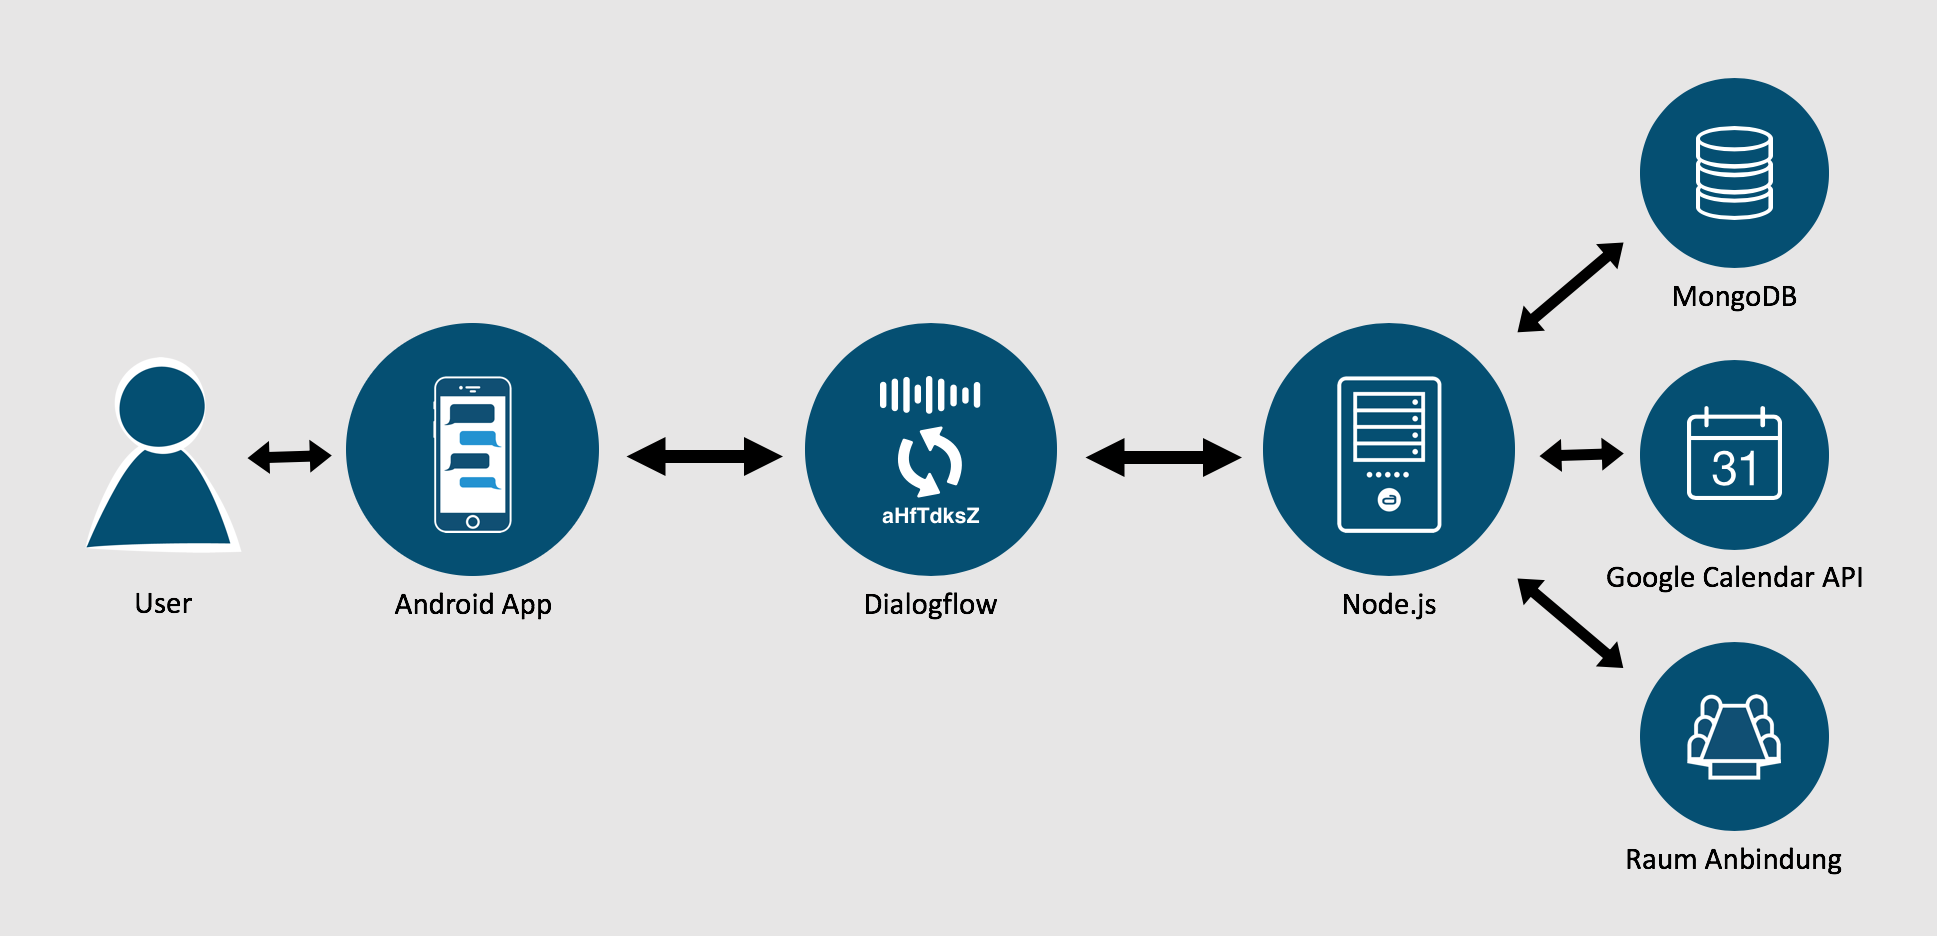
\includegraphics[width=1\textwidth]{bilder/Komponenten-v2.png}
    \caption{Übersicht aller Komponenten ohne Kommunikation}
    \label{fig:komponenten-v2}
\end{figure}

\section{Kommunikation}
\label{sec:kommunikation}

Nachdem im vorangegangenen Kapitel \ref{sec:auswahl-komponenten} die verschiedenen Komponenten beschrieben wurden, stellt sich nun die Frage wie all diese unterschiedlichen Plattformen miteinander kommunizieren. Um dies zu beantworten, werden einige in der Arbeit erprobten Ansätze erläutert und bewertet. 

\subsection{Authentifizierung und Autorisierung}
\label{subsec:authentifizierung-authorisierung}

Wie bereits eingangs erwähnt, nutzt die \adorsys\ den Google-Kalender. Für den Nutzer ist es demnach wünschenswert und komfortabel, wenn er sich in der App auf einer Art \textit{Loginpage} anmelden kann. Genutzt werden können dazu die gewöhnliche E-Mail-Adresse mit der \textit{@adorsys.de}-Endung, welche auf dem Google-Kalender basiert, und das entsprechende Passwort. Der Login innerhalb der App kann für beliebige Anwendungszwecke konfiguriert werden. So lassen sich dabei in der Basisvariante nach erfolgreicher Anmeldung beispielsweise Profilinformationen wie Vor- und Nachname oder der individuelle \ac{ID} eines Nutzers (auch \textit{Person-\ac{ID}}) gewinnen. Je nach Anwendungsfall kann zudem die E-Mail-Adresse oder auch ein \textit{Android-\ac{ID}-Token} erhalten werden. Zu dem Android-\ac{ID}-Token können zusätzlich so genannte \textit{Scopes} hinzugefügt werden, die beispielsweise Lese- oder Schreibzugriff auf den Kalender gewähren. \cite{google_developers_integrating_2018} 

Die erste Idee ist hierbei, bei Anmeldung in der App einen Android-\ac{ID}-Token zu erhalten, der durch alle Komponenten durchgeschleift wird. Dieser würde also über die Textanbindung der App an Dialogflow und deren Verarbeitung im Backend mitgeliefert werden. Damit wäre in jedem Schritt klar, von wem die aktuelle Textnachricht kommt. Außerdem kann jederzeit auf Profilinformationen zugegriffen werden. Bei genauerer Betrachtung treten hierbei zwei wesentliche Probleme auf. Zum einen gibt es keine Möglichkeit, über das Android \ac{SDK} weitere Daten in die Textanfrage an Dialogflow zu stecken. Das \ac{JSON}-File wird anhand des eingegebenen Textes und weiterer Konfigurationen automatisch erzeugt und kann somit nicht modifiziert werden. Ein weiteres Problem stellt sich bei der Authentifizierung mittels Android-\ac{ID}-Token im Backend dar. Aus Sicherheitsgründen ist es nicht möglich, mit einem Token aus einer Android Applikation im Backend auf Kalenderereignisse zuzugreifen \cite{google_developers_authenticate_2018}. 

Für den Zugriff auf Kalenderereignisse im Backend ist nämlich ein eigener, serverseitiger \textit{access token} notwendig. Dieser kann nach dem Aufruf eines Authentifizierungslinks und der Generierung eines Authentifizierungscodes schließlich im Backend erzeugt werden. Mitgeliefert wird dabei noch ein dazugehöriger \textit{refresh token}, der bei Ablauf zur Generierung eines neuen \textit{access token} genutzt werden kann. Außerdem gibt es die Möglichkeit der Verifizierung des Android-\ac{ID}-Tokens im Backend. Über entsprechende Bibliotheken und Methoden kann dabei der Android-\ac{ID}-Token verfiziert und Basis-Profilinformationen wie Name, E-Mail-Adresse oder Person-\ac{ID} herausgefunden werden. 

Zunächst wird noch ein weiterer Ansatz verfolgt. Dabei muss überlegt werden, woran eine Nachricht von bzw. an Dialogflow identifiziert werden kann. Im \ac{JSON}-File von Dialogflow steht neben den Informationen zum geschriebenen Text, dem Intent und verschiedenen Entitäten auch eine \ac{ID} für die aktuelle Session. Diese \textit{Session-\ac{ID}} bleibt dabei im Laufe einer Konversation unverändert und kann somit als \acl{ID} im Backend verwendet werden. Um im Backend zu wissen, zu wem diese Session-\ac{ID} gehört, muss ihr ein weiterer \acl{ID} zugeordnet werden. Denkbar wäre hierbei eine universelle \textit{Device-\ac{ID}} des Geräts. Es gibt dazu mehrere Möglichkeiten, wie beispielsweise eine sogenannte \textit{Unique Telephony Number}, die \textit{MAC-Adresse}, eine \textit{Seriennummer} oder eine \textit{Secure Android-\ac{ID}} \cite{saurel_s._how_2018}. 

Eine dieser Device-\acp{ID} würde dann zusammen mit der Session-\ac{ID} in einer Datenbank liegen, wo sie als gemeinsamer Eintrag miteinander verknüpft werden. Verarbeitet der Server nun im Rahmen des \aclp{DM} eine Nutzeranfrage, kann anhand der Session-\ac{ID} die dazugehörige Device-\ac{ID} aus der Datenbank geholt und somit die Anfrage einem konkreten Nutzer bzw. Gerät zugeordnet werden. Außerdem können zu diesen Einträgen passende Token für den Zugriff auf den Google-Kalender in der Datenbank hinterlegt werden. 

Nachteilig an der Lösung mit der Verknüpfung von Session-\ac{ID} und Device-\ac{ID} ist, dass diese beiden Werte keinerlei Informationen über die Identität des Nutzers geben. Hier kann nun wieder der Google-Login innerhalb der App genutzt werden. Nachdem der User sich erfolgreich angemeldet hat, stehen seine persönlichen Informationen wie Name, E-Mail-Adresse und Person-\ac{ID} zur Verfügung. Nachdem die Person-\ac{ID} universell und für jedes Google-Konto eindeutig ist, kann diese problemlos für den Datenbankeintrag und die damit verbundene Verknüpfung zur Session-\ac{ID} und den Token aus dem Backend verwendet werden. Die Device-\ac{ID} wird damit überflüssig. Im Backend kann die Session-\ac{ID} dann jederzeit über die Abfrage einer Datenbank zugeordnet und entsprechende Daten für die Identität des Users oder seine Token für den Kalenderzugriff gelesen werden. 

Nach ausführlicher Betrachtung stellt sich die Möglichkeit einer Zuordnung des Users durch seine aktuelle Session-\ac{ID} und der Person-\ac{ID} seines Google-Accounts als beste Möglichkeit heraus. Wird der Google-Login innerhalb einer App genutzt, um sich im Backend zu authentifizieren, sollten die Informationen in jedem Fall verschlüsselt übertragen werden \cite{google_developers_authenticate_2018}. Dazu kann der innerhalb der Android App generierte \ac{ID}-Token an den Server gesendet und dort authentifiziert werden. Anschließend können daraus alle notwendigen Profilinformationen exportiert und in einer Datenbank zusammen mit der entsprechenden Session-\ac{ID} gespeichert werden. Möchte der User auf seinen Kalender zugreifen, muss er dies innerhalb der App einmalig mittels einer im Backend generierten \ac{URL} bestätigen. Anschließend werden sein \textit{access token} und \textit{refresh token} in der Datenbank hinterlegt. Aus den vorhergehenden Überlegungen ergibt sich für die Struktur zur Kommunikation zwischen den Komponenten das Schaubild aus Abbildung \ref{fig:komponenten-v3}.
\newline

\begin{figure}[htb]
    \centering
    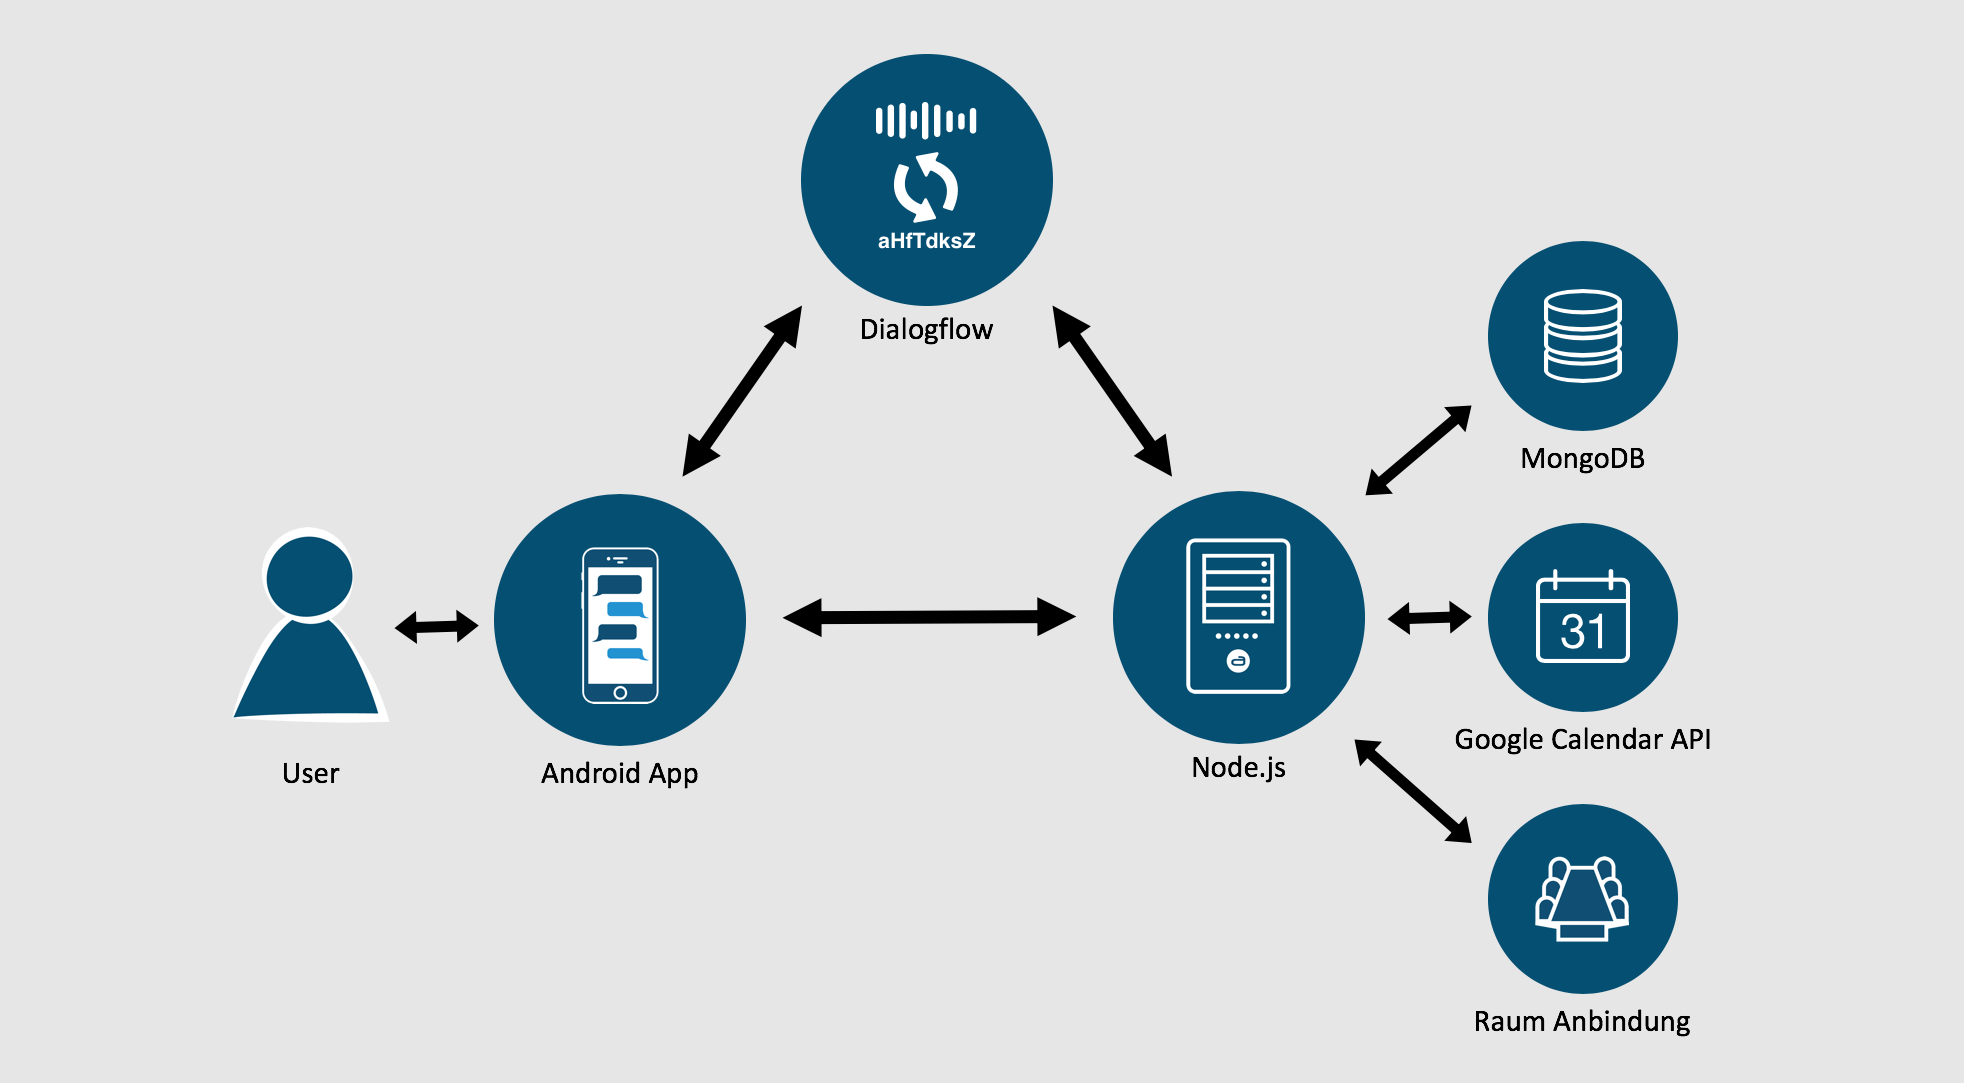
\includegraphics[width=1\textwidth]{bilder/Komponenten-v3.png}
    \caption{Übersicht aller Komponenten mit Kommunikation}
    \label{fig:komponenten-v3}
\end{figure}

\subsection{Schnittstellen}
\label{subsec:Schnittstellen-Konzeption}

Als Schnittstellen zwischen den Komponenten kommen verschiedene Techniken zum Einsatz. Die verwendeten Techniken sollen daher im Folgenden kurz erläutert \mbox{werden}. 

\begin{enumerate}
  \item Von einer Android Applikation aus kann das \textit{Android \ac{SDK} für api.ai}\footnote{api.ai heißt jetzt Dialogflow} genutzt werden, um Anfragen an Dialogflow zu senden \cite{skachkov_dialogflow-android-client:_2018}. Damit können sowohl sprach- als auch textbasierte Anfragen an Dialogflow gesendet und die Antworten ausgewertet werden. 
  
  \item Zur Kommunikation zwischen der Android App und dem Node.js Webservice kann \textit{Retrofit} verwendet werden. Retrofit ist ein \ac{REST} Client für Android und Java und basiert auf der \textit{OkHttp} Bibliothek. Damit ist es möglich, strukturierte Daten (z.B. \ac{JSON}) zu einem \ac{REST}-basierten Webservice zu schicken oder abzurufen. \cite{vogel_using_2018} 
  
  \item Mit Hilfe von \textit{Bespoken} kann eine Verbindung vom Dialogflow Agent auf den lokalen Rechner hergestellt werden. Über einen Proxy-Dienst gibt das Tool eine \ac{URL} aus, welche im Agent als Webhook hinterlegt wird \cite{bespoken_api.ai_2018}. Dies ist allerdings nur so lange relevant, wie der Webservice auf einem lokalen Rechner läuft. Zum einem späteren Zeitpunkt kann hier auf eine \ac{REST}-Schnittstelle zurückgegriffen werden. 
  
  \item Um vom Node.js Webserver aus mit einer MongoDB kommunizieren zu können, kann über \ac{npm} ein \textit{MongoDB Driver} installiert werden. Anschließend kann das entsprechende Modul in den Server eingebunden und über eine \ac{API} darauf zugegriffen werden. \cite{npmjs_mongodb_2018}
  
  \item Der Webservice kann Kalenderereignisse über die \textit{Google Calendar \ac{API}} abfragen oder erstellen. Auch diese wird über ein Modul in Node.js eingebunden. Die Google Calendar \ac{API} basiert wiederum auf \ac{REST} und \ac{HTTP}. \cite{google_developers_node.js_2018}
  
  \item Die Raumanbindung im Backend geschieht ebenfalls über die \textit{Google Calendar \ac{API}}. Die Besprechungsräume sind dabei als Ressourcen in der Domäne der \mbox{\adorsys} angelegt und können nach ihrer Verfügbarkeit abgefragt werden.
  
\end{enumerate}

\clearpage
\section{Android Applikation}
\label{sec:android-applikation}

Wie bereits dem Titel der Arbeit zu entnehmen ist und unter \ref{subsec:frontend} nochmals ausführlich erläutert wird, handelt es sich bei dem Frontend bzw. der Messaging Platform des Systems um eine Android App. Über diese Applikation ist es dem Nutzer möglich, sich im Rahmen des Raumbuchungssystems einzuloggen und anschließend durch die Benutzung eines Chatbots Räume zu reservieren. Im Folgenden soll hierzu ein Überblick gegeben, allerdings nicht detaillierter auf den Quelltext eingegangen werden. Es wird dabei versucht, die Bedienung und den Workflow der App beispielhaft zu verdeutlichen. Dabei ist es leider nicht immer möglich, jeden Arbeitsschritt auf seine kleinste Ebene zu zerlegen. Vielmehr werden die prinzipiellen Abläufe anhand einiger Abbildungen erläutert.

\subsection{Manifest}
\label{subsec:manifest}

Im Android Manifest werden einige grundlegende Informationen deklariert. Nachdem die App über Dialogflow mit dem Internet verbunden sein muss, wird eine entsprechende \textit{Permission} im Manifest verwaltet. Des Weiteren werden hier die beiden Aktivitäten \textit{LoginActivity} und \textit{ChatActivity} eingetragen, wobei die LoginActivity als \textit{Main-} bzw. \textit{Launcher-}Aktivität festgelegt und beim Start der App als erstes aufgerufen wird. Zudem kann hier das Icon der Applikation geändert werden. Das Icon wird vom Nutzer angewählt, wenn er die App auf seinem Smartphone starten möchte und hat eine dementsprechend wichtige Bedeutung. Das Icon\footnote{Das Icon wurde von Mona Kögel entworfen} ist in Abbildung \ref{fig:android-app-icon} dargestellt.
\newline

\begin{figure}[H]
    \centering
    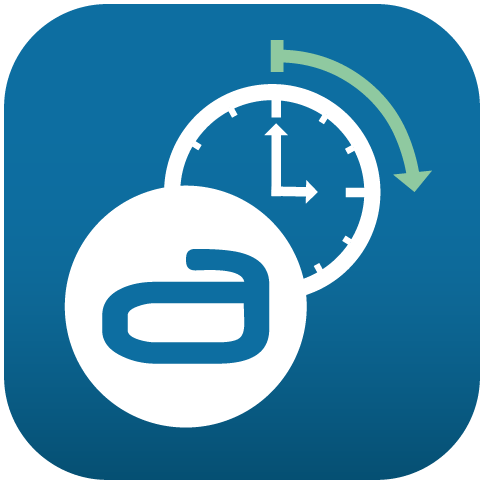
\includegraphics[width=0.2\textwidth]{bilder/AppIcon.png}
    \caption{Icon der Android Applikation}
    \label{fig:android-app-icon}
\end{figure}

\subsection{Anmelden}
\label{subsec:login-activity}

Nach erstmaligem Start der Applikation findet sich der Nutzer auf einer \textit{Loginpage} wieder. Der Login wurde gemäß der offiziellen Dokumentation zum \textit{Google Sign-In für Android Applikationen} integriert \cite{google_developers_integrating_2018}. Abbildung \ref{fig:android-login-screen} zeigt die relevanten \mbox{Anmeldebildschirme}. 

Auf der linken Seite ist der Startbildschirm zu sehen. Betätigt der Nutzer den Button \textit{Sign in}, kann er aus seinen mit dem Android-Device verknüpften Google-Accounts wählen oder einen weiteren beliebigen Account verknüpfen. Nach erfolgreicher Anmeldung steht anschließend ein \textit{Android-\ac{ID}-Token} zur Verfügung, der wie bereits unter \ref{subsec:authentifizierung-authorisierung} beschrieben, im Backend verifiziert werden kann. Erwähnenswert ist in diesem Zusammenhang, dass dieser Login mit allen Google-Konten funktioniert, eine tatsächliche Raumbuchung im späteren Verlauf allerdings nur mit Accounts innerhalb der Domäne der \adorsys\ möglich ist. Ist der Nutzer erfolgreich eingeloggt, ändert sich der \textit{Login Status} auf dem Screen und der User wird automatisch zum Chatbot weitergeleitet.
\newline

\begin{figure}[H]
    \centering
    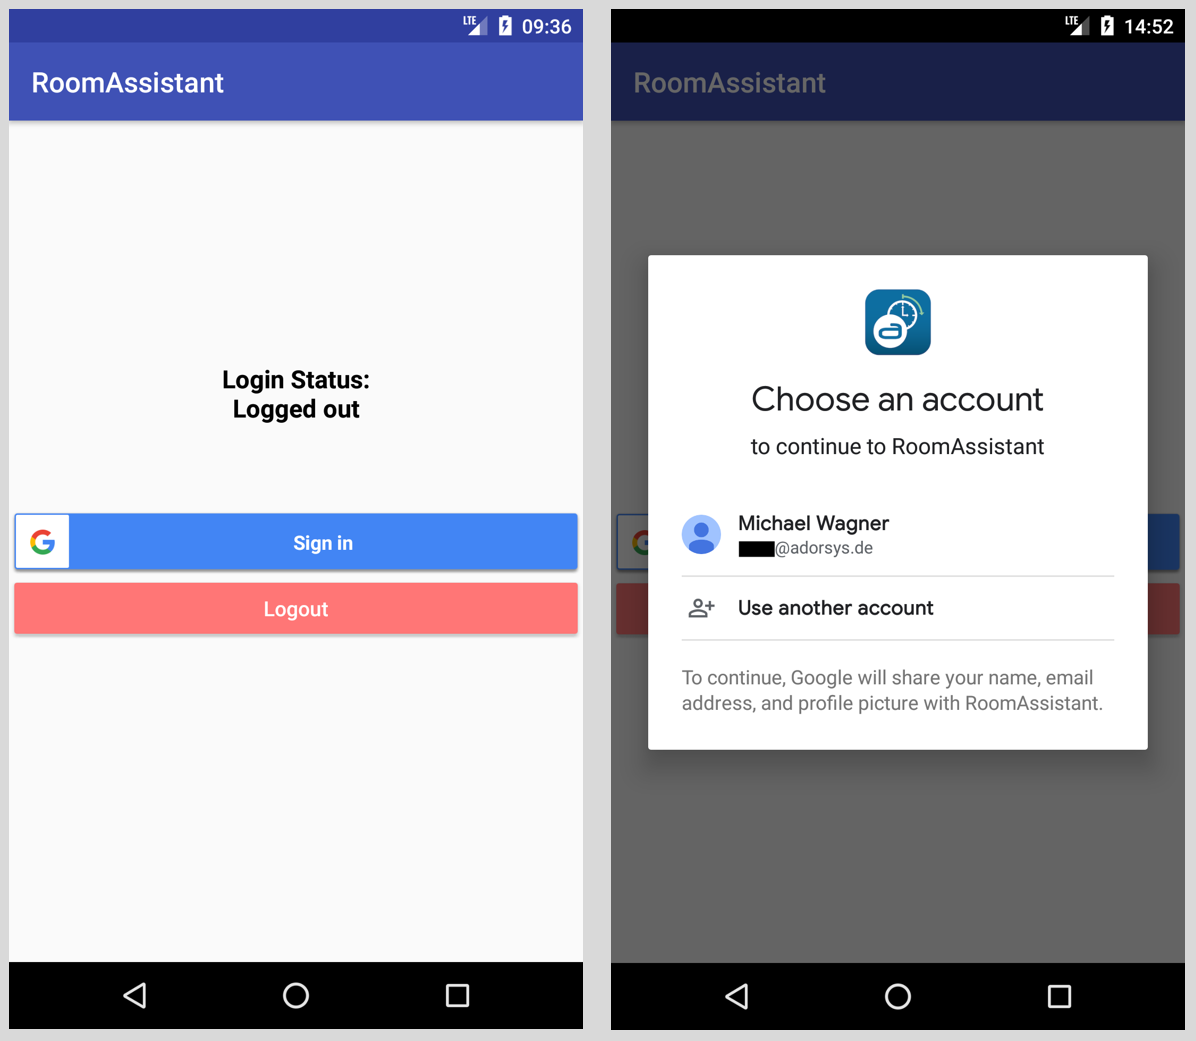
\includegraphics[width=0.8\textwidth]{bilder/LoginScreenCombined.png}
    \caption{Benutzeroberfläche zum Anmelden in der Android Applikation}
    \label{fig:android-login-screen}
\end{figure}

\FloatBarrier
\subsection{Kalenderzugriff}
\label{subsec:authorization-prozess}

Beim Start der \textit{ChatActivity} wird zunächst, vom Nutzer unbemerkt, eine Art \textit{Handshake} durchgeführt. Die Applikation sendet einen Request mit der Query \textit{Hallo} an Dialogflow. Über den Webhook kann diese Anfrage dann im Node.js Webservice ausgewertet werden. Anhand der mitgelieferten Daten können die dazugehörigen Nutzereinträge aus der Datenbank gelesen werden. In diesem Zuge wird auch direkt der Eintrag für die aktuelle Session-\ac{ID} aktualisiert. Anschließend wird geprüft, ob bereits ein gültiger \textit{access token} in der Datenbank vorhanden ist. Eine entsprechende \ac{JSON}-Response wird zunächst zurück an Dialogflow und von dort aus zurück zur Android App gesendet. Abbildung \ref{fig:sequence-diagramm-authorization-flow} verdeutlicht diesen Prozess durch die Darstellung eines entsprechenden Sequenzdiagramms.
\newline

\begin{figure}[H]
    \centering
    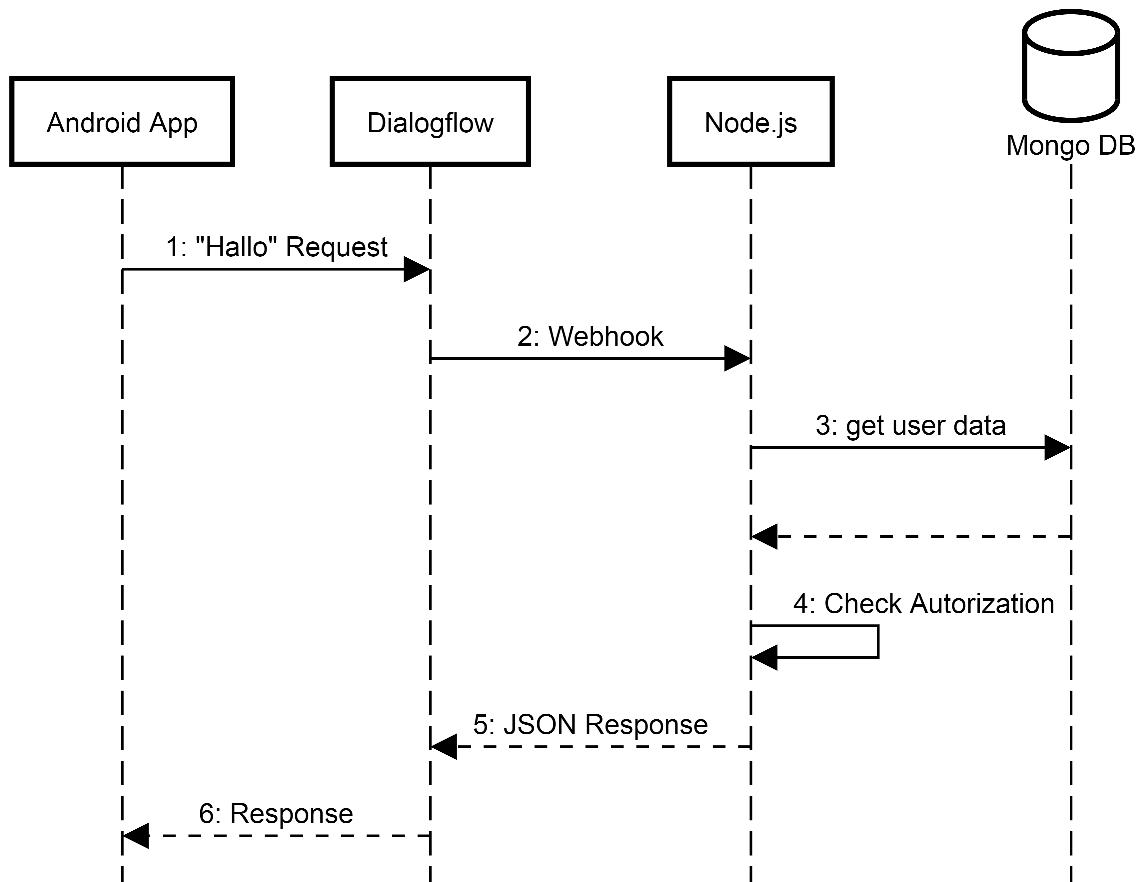
\includegraphics[width=0.9\textwidth]{bilder/Authorization-Flow.png}
    \caption{Sequenzdiagramm zur Autorisierung}
    \label{fig:sequence-diagramm-authorization-flow}
\end{figure}

Ist der User noch nicht autorisiert, wird er durch eine entsprechende Response dazu aufgefordert. Diese Abfolge ist in Abbildung \ref{fig:android-authorization-screen} festgehalten. Innerhalb der \textit{ChatActivity} öffnet sich in diesem Zusammenhang ein Browserfenster (linker Screen), in dem sich der Nutzer anmelden und Zugriff auf seinen Kalender gewähren kann (mittlerer Screen). Hat er dies getan, erhält er einen \textit{Authorization Code}, den er dem Chatbot anschließend zuschickt (rechter Screen). Im Backend wird der entsprechende Code geprüft, der \textit{access token} bzw. \textit{refresh token} generiert und in der Datenbank hinterlegt. Der Chatbot vermeldet dem Nutzer die Nachricht, dass die Autorisierung erfolgreich war. Beim nächsten Konversationsstart kennt der Chatbot den Nutzer und begrüßt ihn mit Phrasen wie \textit{„Hey, willkommen zurück“} oder \textit{„Schön dich zu sehen. Was kann ich für dich tun?“}.
\newline

\begin{figure}[H]
    \centering
    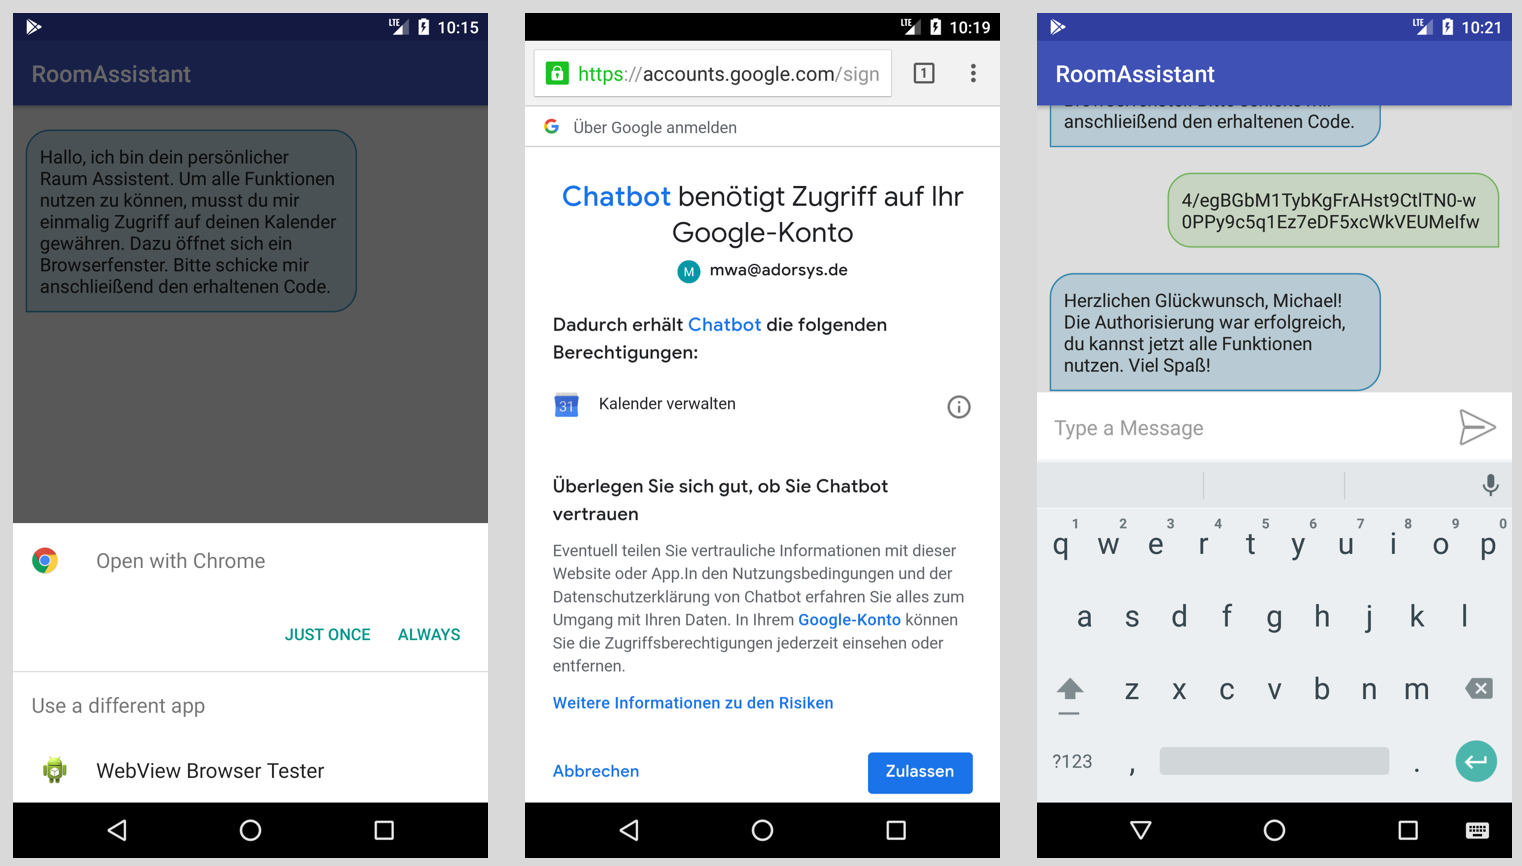
\includegraphics[width=0.9\textwidth]{bilder/AuthorizationScreenCombined.PNG}
    \caption{Benutzeroberfläche zum Autorisieren in der Android Applikation}
    \label{fig:android-authorization-screen}
\end{figure}

\FloatBarrier
\subsection{Chat Interface}
\label{subsec:Chat Interface}

Die \textit{ChatActivity} bzw. das \textit{Chat Interface} stellt das Kernelement der Android Applikation dar. Es besteht im Prinzip aus einer \textit{RecyclerView}, einem \textit{EditText} Feld und einem  \textit{Button}. Diese sind durch mehrere, verschachtelte \textit{RelativeLayouts} so angeordnet, dass sich Eingabefeld und Sendebutton immer am unteren Rand befinden. Bei Eingabe einer Nachricht durch den Nutzer klappt sich eine Tastatur auf und die RecyclerView passt sich entsprechend an. In die RecyclerView können verschiedene Elemente nach und nach eingeschoben werden, sodass für den Nutzer am Ende ein chronologischer und scrollbarer Nachrichtenverlauf sichtbar wird. Dieses Prinzip wurde zuvor bereits im rechten Screen der Abbildung \ref{fig:android-authorization-screen} dargestellt. 

Die \ac{UI}-Erweiterungen sind dabei in einer eigenen \ac{XML}-Datei definiert und werden codeseitig von einer Art \textit{Adapter} verwaltet. Dieser Adapter beinhaltet eine Liste mit Instanzen einer eigenen Klasse \textit{ChatMessage}. Eine Chatmessage hat üblicherweise je ein Attribut für den \textit{Content} und den \textit{Type}. Der Content beschreibt den anzuzeigenden Text, während der Type angibt um welche Art von Nachricht es sich handelt. Aufgrund des Umfangs und der begrenzten Zeit wurden in der Arbeit nur einige im Rahmen der Konzeption entstandenen \ac{UI}-Erweiterungen umgesetzt. Diese werden in Tabelle \ref{tab:arten-nachrichten-chat-interface} genauer erläutert.
\newline

\begin{table}[!htb]
\centering
 \begin{tabular}{ | C{4cm} || C{1.5cm} || C{5cm} || C{2cm} |} 
 \hline
 Type & Art & Beschreibung & Orientierung \\
 \hhline{=::===}
 \hline MSG\_SENT & Text & Textnachricht User & rechts \\ 
 \hline MSG\_RECEIVED & Text & Textnachricht Chatbot & links \\ 
 \hline BUTTON\_YES\_NO & Buttons & Textnachricht mit Buttons ja/nein & links \\ 
 \hline SLIDER\_DURATION & Slider & Textnachricht mit Slider für Dauer & links \\ 
 \hline
\end{tabular}
\caption{Arten von Nachrichten im Chat Interface}
\label{tab:arten-nachrichten-chat-interface}
\end{table}

Diese Unterscheidung macht es möglich, der RecyclerView je nach Ausgangspunkt unterschiedliche \ac{UI}-Elemente hinzuzufügen. Ein beispielhafter Konversationsablauf mit allen implementierten \ac{UI}-Elementen ist in Abbildung \ref{fig:android-chat-interface-screen} dargestellt. 

Sendet der User eine Textnachricht an den Chatbot, erscheint seine rechtsbündige Textnachricht mit entsprechender farblicher Kennzeichnung. Entsprechendes gilt analog für die Textnachrichten des Chatbots. Auch das Feature \textit{Chatbot is thinking} kann somit implementiert werden. Dazu wird nach Abschicken der Nutzeranfrage an Dialogflow eine Textnachricht vom Typ \textit{MSG\_RECEIVED} in die RecyclerView geschoben. Diese bleibt dort so lange, bis die Antwort vom Backend und über Dialogflow zurück kommt. 

Dies dauert je nach Komplexität in der Regel wenige Sekunden. Der Nutzer erhält also direkt Feedback, dass seine Anfrage bearbeitet wird. Wurde die Response erhalten, kann das Element wieder entfernt werden und je nach Nachrichtenart die tatsächliche Rückmeldung des Systems angezeigt werden. Slider oder Buttons lassen sich nun wie gewohnt bedienen. Wird eine Auswahl über einen Button bestätigt, senden die \textit{onClick} Ereignisse eine Nachricht in textueller Form an Dialogflow und der Ablauf beginnt wieder von vorne. 

Da alle Eingaben des Nutzers über Dialogflow laufen und dort in Form einer \mbox{Textquery} ankommen müssen, lässt sich das System auch jederzeit über das Texteingabefeld bedienen. Die \ac{UI}-Erweiterungen dienen lediglich als Vorschlag und Angebot durch das System und sollen gegebenenfalls die Bedienung des Chatbots erleichtern.
\newline

\begin{figure}[H]
    \centering
    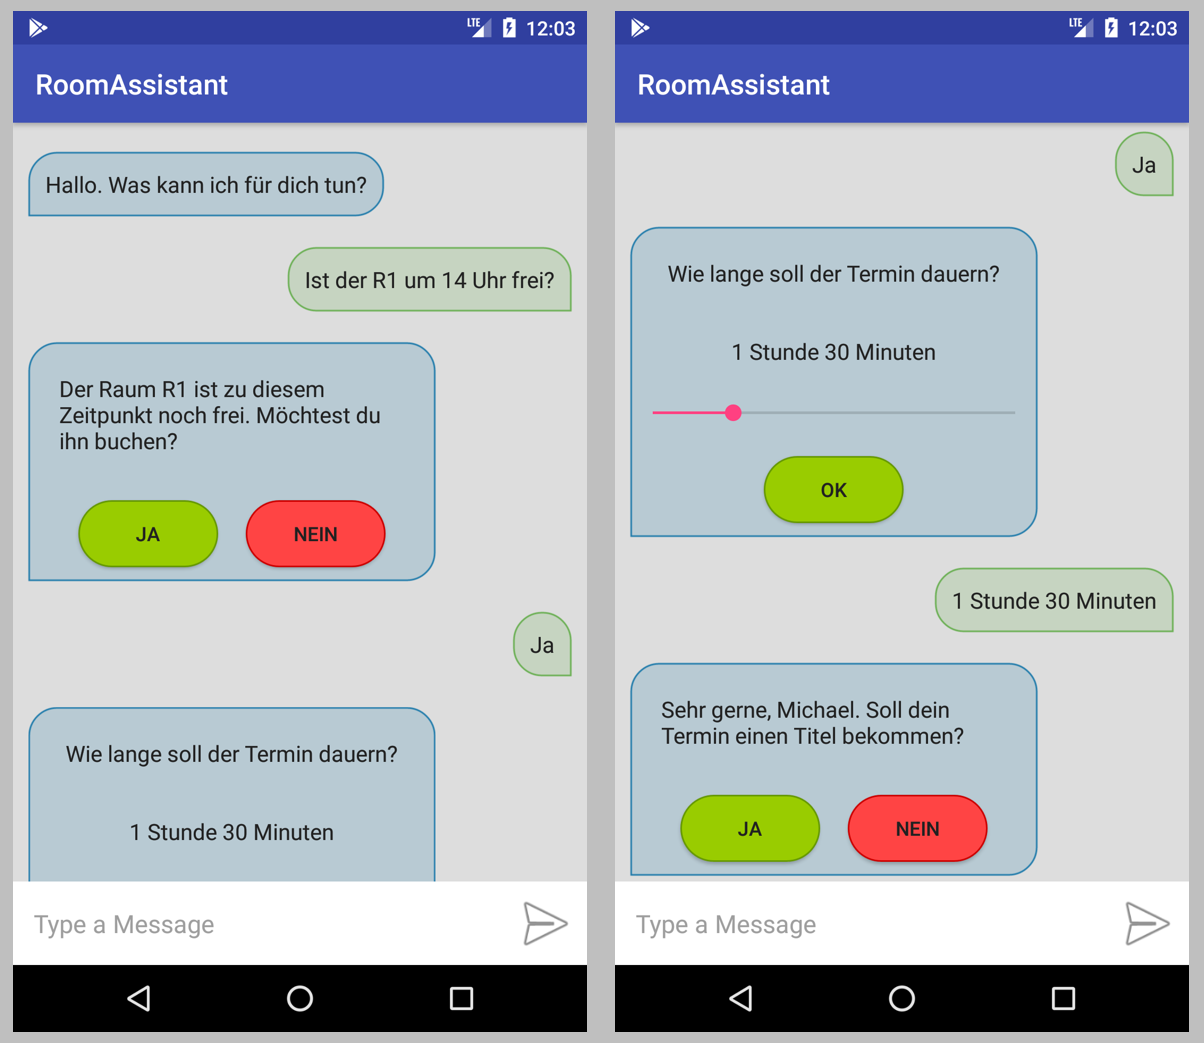
\includegraphics[width=0.9\textwidth]{bilder/ChatInterfaceCombined.png}
    \caption{Chat Interface in der Android Applikation}
    \label{fig:android-chat-interface-screen}
\end{figure}

Es ist nicht immer leicht, das Prinzip und den Umgang mit einer mobilen Applikation nur durch textuelle Beschreibung und Abbildungen darzustellen. Um die Bedienung und den Workflow der Android Applikation greifbarer zu machen, befinden sich auf der CD im Anhang einige \textit{Videos} zum beispielhaften Ablauf einer \textit{Autorisierung}, \textit{Raumbuchung} oder \textit{-abfrage}.



\clearpage
\section{Dialogflow Agent}
\label{sec:dialogflow-agent}

Nach dem ausführlichen Vergleich verschiedener \ac{NLP}-Plattformen in  \ref{subsec:nlp-plattform} fiel die Wahl auf Dialogflow. Die prinzipielle Aufgabe der \ac{NLP}-Plattform ist es, die Intents und Entitäten der Nutzeranfrage zu erkennen und richtig zuzuordnen. Außerdem ist Dialogflow für einen möglichst flüssigen Konversationsflow zuständig. All diese Aufgaben kombiniert in diesem Zusammenhang ein so genannter \textit{Agent}. 

Abbildung \ref{fig:dialogflow-agent-overview} zeigt den prinzipiellen Aufbau eines \textit{Dialogflow Agents} (orange Komponenten). Im Grunde kann dieses Strukturbild analog zu der Abbildung \ref{fig:komponenten-v2} betrachtet werden. 
\newline

\begin{figure}[H]
    \centering
    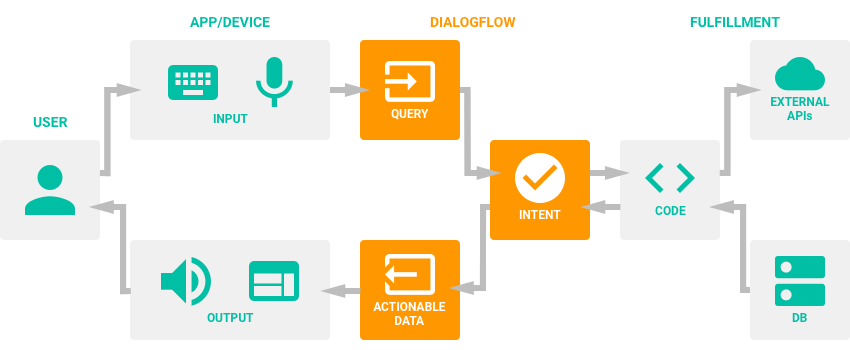
\includegraphics[width=0.9\textwidth]{bilder/dialogflow-agent.png}
    \caption{Prinzipieller Aufbau eines Dialogflow Agents \cite{google_cloud_agents_2018}}
    \label{fig:dialogflow-agent-overview}
\end{figure}

Die linke Seite stellt den User inklusive seiner Ein- und Ausgabemöglichkeiten dar. Im Rahmen der Arbeit ist dies die zuvor beschriebene Android Applikation. Direkt danach ist der Dialogflow Agent anzuordnen. Er erhält eine Query, also die Nutzeranfrage in Textform, ordnet diese einem Intent zu und zieht die relevanten Entitäten heraus. Das hier als \textit{Fulfillment} bezeichnete stellt im Rahmen der Arbeit das Backend dar. Hier werden die Intents und Entitäten ausgewertet und externe \acp{API} oder Datenbanken angebunden. Eine entsprechende Response gelangt dann auf dem Rückweg wiederum über Dialogflow an den User. 

\subsection{Intents}
\label{subsec:agent-intents}

Aufgrund der begrenzten Zeit liegt der Fokus in der Implementierung auf der grundlegenden Funktion. Dazu soll es möglich sein, über das \acl{CUI} nach freien Räumen zu suchen und diese zu reservieren. Auch die Umsetzung der Intents wird daher auf diese beiden Fälle beschränkt. Zudem gibt es standardmäßig bei der Erstellung eines \textit{Agents} je einen \textit{Default Welcome Intent} zur Begrüßung und einen \textit{Default Fallback Intent} als Absicherung, wenn der Chatbot den Nutzer nicht verstanden hat. Um die verschiedenen Intents und Abläufe etwas konkreter darstellen zu können, sind diese in Abbildung \ref{fig:dialogflow-agent-structure} zusammengefasst. Die Abbildung dient der Verdeutlichung des Workflows und stimmt daher nicht eins zu eins mit dem tatsächlichen Agent überein. 
\newline

\begin{figure}[H]
    \centering
    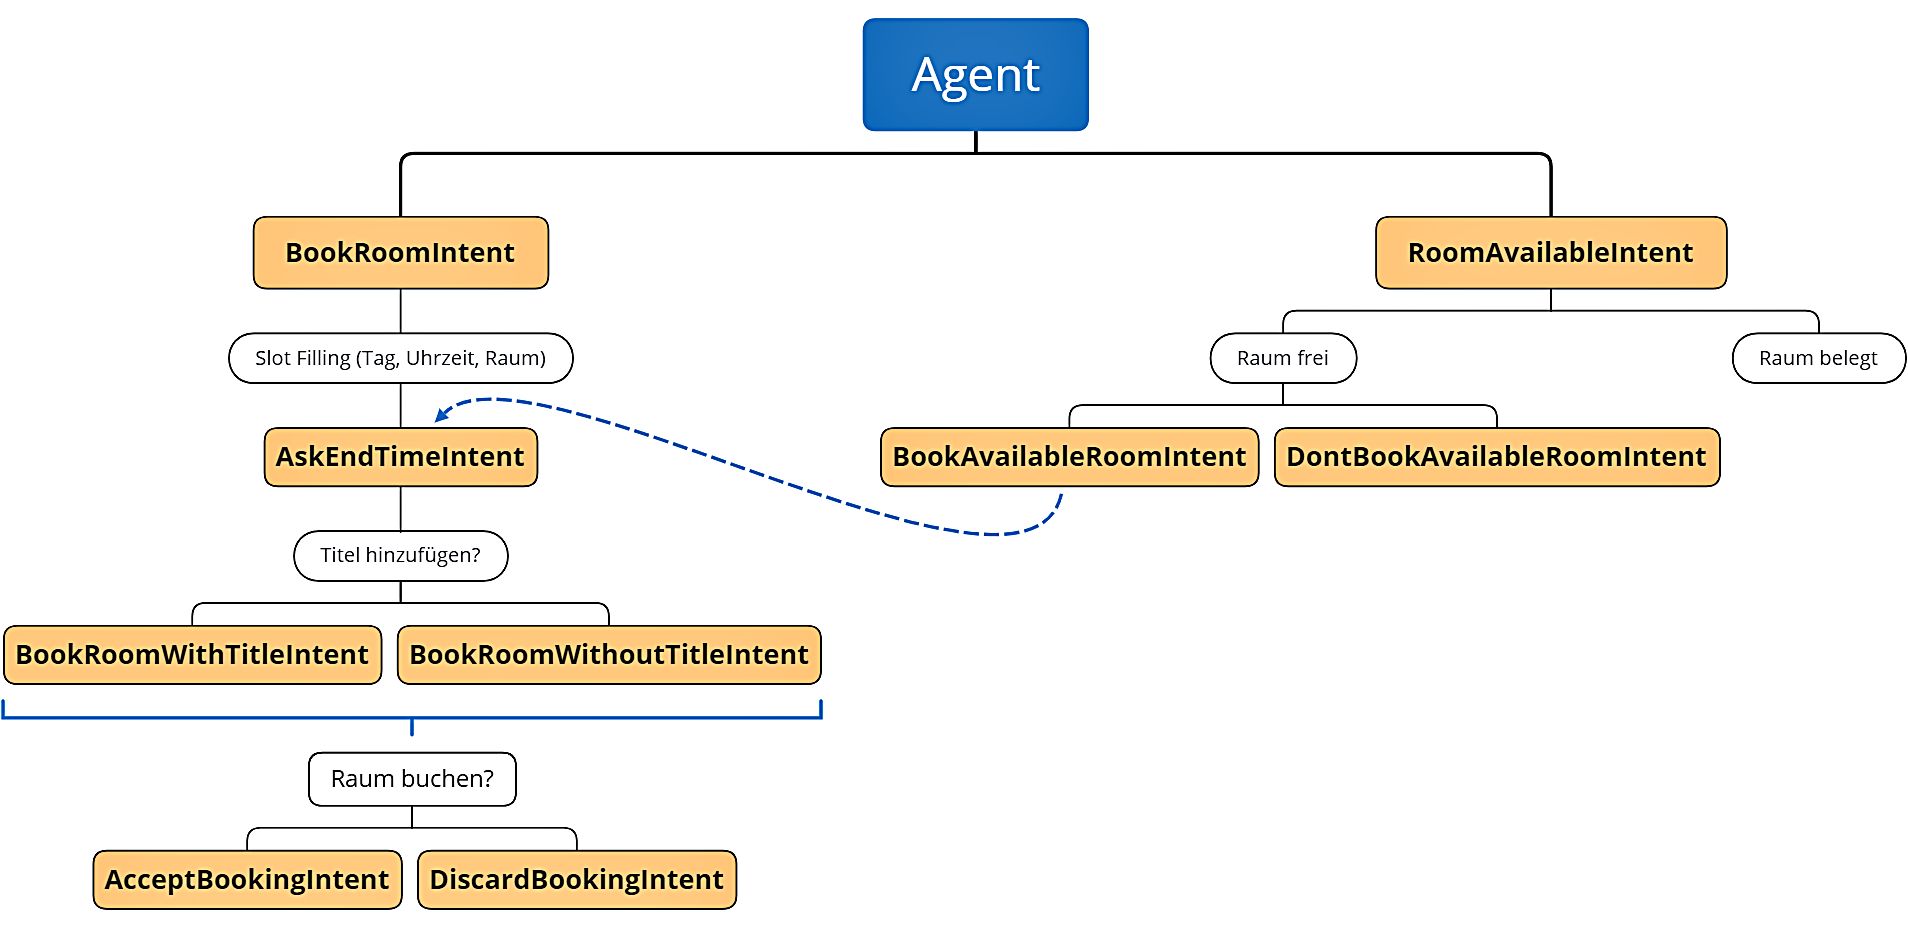
\includegraphics[width=1\textwidth]{bilder/DialogflowIntentStructure_win.PNG}
    \caption{Struktur der Intents im Dialogflow Agent}
    \label{fig:dialogflow-agent-structure}
\end{figure}

Zur Realisierung der Raumbuchung gibt es die beiden Intents \textit{BookRoomIntent} und \textit{RoomAvailableIntent}. Erkennt der Chatbot, dass der Nutzer einen Raum buchen möchte, findet zunächst ein so genanntes \textit{Slot Filling} statt. Dabei werden nach und nach alle für die Buchung notwendigen Parameter abgefragt. Ohne diese Parameter kann im Backend keine Aussage getroffen werden, ob ein oder mehrere Räume zu diesem Zeitpunkt noch frei sind. Ist eine Anfrage in sofern verifiziert, dass alle nötigen Parameter vorhanden sind und der Raum frei ist, springt der Agent in den \textit{AskEndTimeIntent}. Hier wird der Nutzer dann gebeten, eine Endzeit oder Dauer des Termins anzugeben. Anschließend wird noch eine Festlegung zum Titel des Termins getroffen. Wie bereits vorher festgelegt, müssen alle Termine ab 1,5 Stunden einen spezifischen Titel haben. Für kürzere Meetings ist die Angabe eines Titels optional. Möchte der User keinen Titel angeben, wird vom System ein Standardtitel mit der E-Mail-Adresse des Organisators eingetragen. Vor der endgültigen Buchung gibt es noch eine Art \textit{Confirm Message}, mit der der Nutzer die Buchung final bestätigt. 

Möchte der Nutzer dagegen zunächst nur nach einem oder mehreren freien Räumen suchen, wird dies über den \textit{RoomAvailableIntent} realisiert. Wird explizit nach einem Raum gefragt oder ist zu dem gewählten Zeitpunkt nur ein Raum frei, besteht für den User die Möglichkeit, durch einen einfachen Buttonklick direkt in die Buchung des Raums zu springen. Ab hier wiederholt sich dann der zuvor beschriebene Ablauf nach dem \textit{AskEndTimeIntent}. 

\subsection{Entitäten}
\label{subsec:agent-entities}

Im Kontext der Raumbuchung kommen viele, verschiedene Entitäten vor. Wie in Tabelle \ref{tab:nlp-plattform-vergleich} untersucht, werden die relevanten Parameter schon als so genannte \textit{System Entities} von Dialogflow mitgeliefert \cite{dialogflow_system_2018}. Eine Ausnahme stellt hierbei die Entität für den Raum dar. In Dialogflow ist es allerdings problemlos möglich, eigene Entitäten, so genannte \textit{Developer Entities} zu definieren. In der Tabelle \ref{tab:agent-entities} sind alle im Rahmen des Agents verwendeten Entitäten aufgeführt. 
\newline

\begin{table}[H]
\centering
 \begin{tabular}{ | C{2.5cm} || C{1.5cm} || C{4.5cm} || C{4cm} |} 
 \hline
 Name & Art & Beispiel & Beschreibung \\
 \hhline{=::===}
 \hline @sys.date & System & 2018-10-17T12:00:00+02:00 & Datum (ISO-8601)\\ 
 \hline @sys.time & System & 2018-10-17T16:30:00+02:00 & Uhrzeit (ISO-8601)\\ 
 \hline @sys.duration & System & \{"'amount"':1,"'unit"':"'stunde"'\} & Dauer als Objekt \\
 \hline @sys.any & System & Vorstellungsgespräch & Beliebiger Terminname \\ 
 \hline @RoomEntity & Developer & R1 & Name des Raumes \\ 
 \hline
\end{tabular}
\caption{Übersicht der Entitäten des Dialogflow Agents}
\label{tab:agent-entities}
\end{table}

Die Systementitäten \textit{date} und \textit{time} müssen getrennt betrachtet werden. Beide liefern einen Zeitstempel im \textit{ISO-8601 Format}. Im Backend wird dann aus der Information für Datum und Uhrzeit ein kombinierter Zeitstempel errechnet. Für die Dauer des Termins kann der Typ \textit{duration} verwendet werden. Dieser liefert ein Objekt mit einem Integer für den Wert und einem String für die Einheit. Als Titel kann über den Typ \textit{any} ein beliebiger Text eingegeben werden. Die selbst erstellte Entität für die verschiedenen Räume kann den Namen jedes Besprechungsraums beinhalten. Weiterhin gibt es hierbei den Wert \textit{RX}, falls der Nutzer keinen bestimmten Raum buchen möchte.

\section{Node.js Webservice}
\label{sec:nodejs-webservice}

Wie bereits in \ref{subsec:webservice} beschrieben, wird für die Implementierung des Backends Node.js verwendet. Auf das Backend kommen in diesem Fall mehrere Aufgaben zu. Es erhält über einen so genannten Webhook ein von Dialogflow generiertes \ac{JSON}-Objekt. In diesem Objekt sind alle für die aktuelle Session relevanten Daten aufgelistet. Da nicht alle von Dialogflow mitgelieferten Daten relevant sind, wird zunächst über einen \textit{Callback} ein Objekt generiert, in dem alle relevanten Daten zur Useranfrage abgelegt sind. Die relevanten Daten sind in Tabelle \ref{tab:data-dialogflow-json} aufgelistet.
\newline

\begin{table}[H]
\centering
 \begin{tabular}{ | C{3cm} || C{1.5cm} || C{8cm} |} 
 \hline
 Name & Art & Beschreibung \\
 \hhline{=::==}
 \hline session\_id & String & Identifier zur Zuordnung zu User aus Datenbank \\ 
 \hline intent\_id & String  & Eindeutiger Identifier für den Intent \\ 
 \hline intent\_name & String & Name des Intents \\
 \hline parameters & Object  & Sämtliche relevante Parameter, z.B. time, date, etc. \\ 
 \hline
\end{tabular}
\caption{Relevante Daten aus Dialogflow \acs{JSON}-Request}
\label{tab:data-dialogflow-json}
\end{table}

Weiterhin wird eine Datenbankanbindung benötigt, in der die Daten der User gespeichert und verwaltet werden. Die Zuordnung im Rahmen der Anfragen von Dialogflow geschieht durch die Session-\ac{ID}. Jeder Datenbankeintrag besitzt eine universelle \mbox{Person-\ac{ID}}, über die der Eintrag einem User zugeordnet werden kann. Zudem sind die E-Mail-Adresse und der Vorname des Nutzers hinterlegt. Über die abgespeicherten Token kann anschließend ein Zugriff auf die Kalenderereignisse stattfinden. Der Wert für das \textit{expiry date} dient dem internen Handling zur Überprüfung der Gültigkeit und Erneuerung des \textit{access token}. Eine Übersicht aller Parameter zu einem Nutzereintrag in der Datenbank ist in Tabelle \ref{tab:data-datenbank} dargestellt.
\newline

\begin{table}[H]
\centering
 \begin{tabular}{ | C{3cm} || C{1.5cm} || C{7cm} |} 
 \hline
 Name & Art & Beschreibung \\
 \hhline{=::==}
 \hline session\_id & String & Identifier zur Zuordnung des Users \\ 
 \hline person\_id & String & Eindeutiger Identifier des Google-Accounts \\ 
 \hline email & String & E-Mail-Adresse des Users \\ 
 \hline given\_name & String & Vorname des Users \\ 
 \hline access\_token & String & Zugriffs Token des Users \\ 
 \hline refresh\_token & String & Refresh Token des Users \\
 \hline expiry\_date & Number  & Ablaufdatum des Tokens \\ 
 \hline
\end{tabular}
\caption{Parameter aus der Datenbank}
\label{tab:data-datenbank}
\end{table}

Die Anbindung der \textit{Google Calendar \ac{API}} zum Abfragen und Erstellen von Terminen ist ebenso Aufgabe des Webservices. Die Google Calendar \ac{API} kann dabei sowohl für den Eintrag in den Kalender des Users, als auch für die Abfrage der Besprechungsräume im Office der \adorsys\ verwendet werden. Die Räume sind dabei als Ressourcen innerhalb der Domäne der Firma angelegt und über eine kryptische E-Mail-Adresse ansprechbar. Abfragen von freien Zeiträumen und Einträge in die Terminkalender können dann gemäß \cite{google_developers_node.js_2018} und \cite{google_developers_create_2018} getätigt werden.

Um die Einträge in der Datenbank auf dem aktuellen Stand zu halten, müssen die aktuelle Session-\ac{ID} und der zum Nutzer gehörige Android-\ac{ID}-Token über eine \ac{HTTP}-Nachricht von der Android App an das Backend geschickt werden. Auf die gleiche Weise wird auch der Authentifizierungscode versendet, aus dem anschließend im Backend die Token für den Kalenderzugriff generiert werden. Für diese Funktionalitäten werden im Backend so genannte Endpunkte definiert. Um dies zu realisieren wird das Node.js-Framework \textit{Express} verwendet. Damit kann relativ einfach und minimalistisch eine \ac{REST}-Schnittstelle umgesetzt werden. Es wird dazu jeweils eine \textit{POST-Methode} zum Verifizieren von Session-\ac{ID} und Android-\ac{ID}-Token, sowie der Auswertung des Authentifizierungscodes implementiert.

Im Backend findet mit den von Dialogflow gelieferten Daten sozusagen das \acl{DM} statt. Welches \ac{UI}-Element die Android App am Ende als Antwort für den User anzeigen soll, ist durch ein \ac{JSON}-Objekt definiert. Dabei gibt es die Möglichkeit, Daten über einen so genannten \textit{payload} durch Dialogflow durchzuschleifen. Ein Beispiel der Darstellung des \ac{UI}-Elements im Backend zeigt Listing \ref{lst:json-payload}.
\newline

\begin{lstlisting}[caption={Darstellung des \acs{UI}-Elements im Backend im \acs{JSON}-Format}, captionpos=b, label={lst:json-payload}, language=myjson]
"payload": 
{
    "android": 
	 {
        "type": "button",
        "text": "Soll dein Termin einen Titel haben?"
	 }
}
\end{lstlisting}

Zur Unterscheidung der unterschiedlichen \ac{UI}-Elemente dient hierbei der \textit{type}. In Listing \ref{lst:json-payload} ist dies ein \textit{button}, der im Frontend eine Phrase und die Auswahlbuttons \textit{Ja}/\textit{Nein} darstellt. Der \textit{text} repräsentiert an dieser Stelle die Phrase, die der Nutzer als Antwort erhält und ist für alle \ac{UI}-Elemente notwendig. Anstelle von \textit{button} kann an dieser Stelle auch \textit{textmessage} oder \textit{slider} angegeben werden. Die Zuordnung ist analog zu der im Unterkapitel \nameref{subsec:Chat Interface} angegebenen Tabelle \ref{tab:arten-nachrichten-chat-interface}.

Auf diese Art und Weise können nun beliebig viele, weitere \ac{UI}-Elemente definiert und umgesetzt werden. Dabei muss natürlich das entsprechende \ac{UI}-Element auch in der Android App bekannt und implementiert sein. Als erstes Modell und zum Datenaustausch funktioniert dies auch problemlos. Jedoch erscheinen zukünftige Probleme nicht unvermeidbar. Über die gewählte Architektur und den Komponentenaufbau aus \ref{sec:auswahl-komponenten} müssen die entsprechenden Daten immer durch Dialogflow hindurch geschleust werden. Ändert sich hierbei der Aufbau des \ac{JSON}-Objekts oder wird gar das Durchschleifen von Daten unterbunden, so muss die gewählte Vorgehensweise geändert werden oder ist im schlimmsten Fall gar nicht mehr realisierbar. Als Anregung sei in diesem Zusammhang erwähnt, dass die Komponenten \textit{Webservice} und \textit{\ac{NLP}-Plattform} in ihrer Anordnung auch vertauscht werden könnten. Dies hätte den Vorteil, dass Dialogflow nur noch für das \textit{\acl{NLU}} zuständig wäre und keine Daten darüber mitgeschleift werden müssen. Diese Ansätze werden allerdings nicht weiter beleuchtet, sondern dienen lediglich als kritische Hinterfragung der eigenen Struktur.

Abschließend sollen alle für das System relevanten Komponenten und der damit verbundene Ablauf vom Senden einer Nachricht durch den User bis zur Rückmeldung einer Nachricht in der App anhand eines Sequenzdiagramms dargestellt werden. Anzumerken ist hierbei, dass dieses Diagramm natürlich nicht für alle Anwendungsfälle gleich ist. Es soll vielmehr die Hintergründe anhand eines typischen und häufig vorkommenden Use Cases, wie beispielsweise der Abfrage eines freien Raumes, verdeutlichen. Das entsprechende Sequenzdiagramm ist in Abbildung \ref{fig:sequence-diagramm-basic-system-interaction} dargestellt.
\newline

\begin{figure}[H]
    \centering
    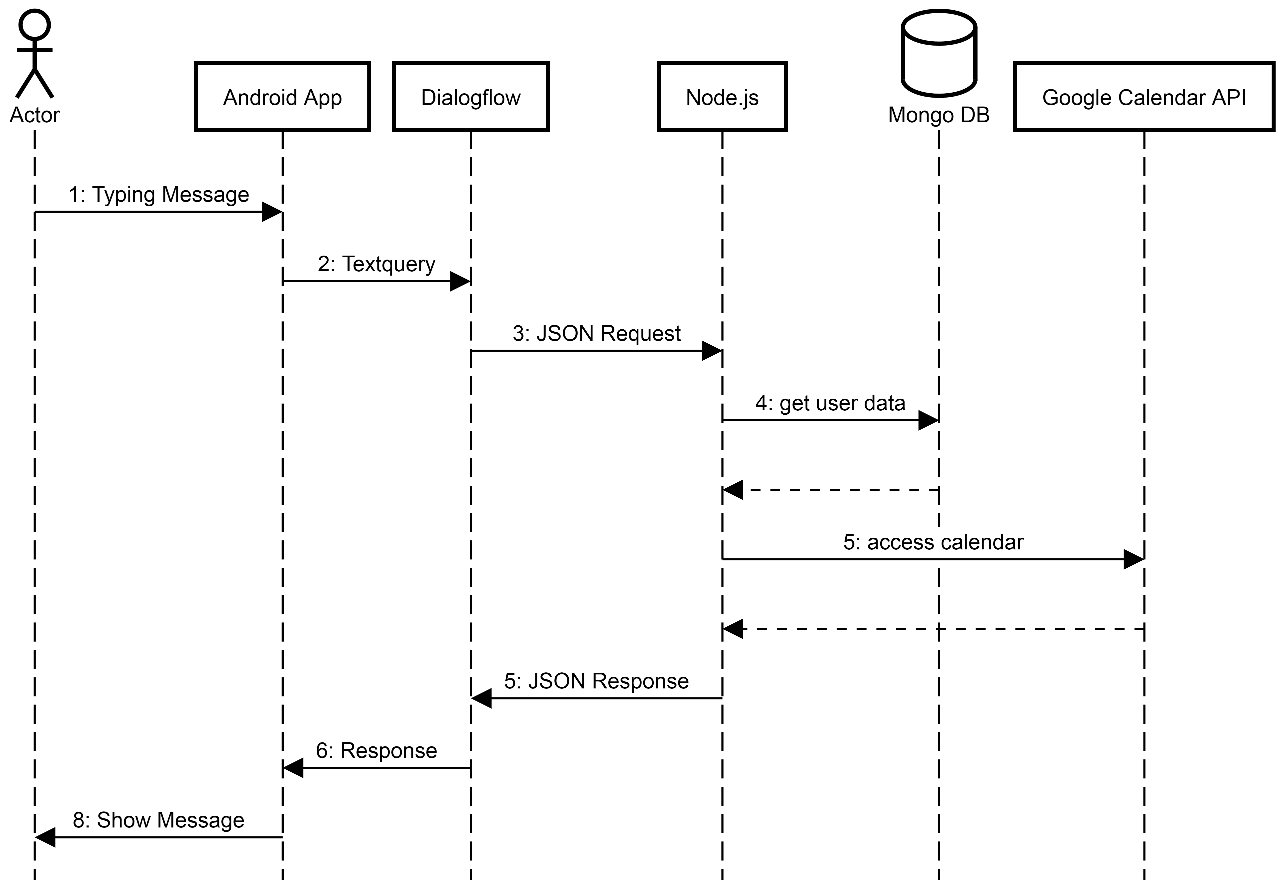
\includegraphics[width=1\textwidth]{bilder/Basic-System-Interaction.png}
    \caption{Sequenzdiagramm zur Interaktion der Systeme}
    \label{fig:sequence-diagramm-basic-system-interaction}
\end{figure}

In der Android Applikation tippt der User zunächst eine Nachricht ein oder bedient sich eines bereits vorhandenen \ac{UI}-Elements und sendet so eine textuelle Nachricht an Dialogflow. Dort wird die Nachricht mit Hilfe von \acl{NLU} interpretiert und gelangt über den Webhook an den Node.js Server. Anhand der hinterlegten Session-\ac{ID} können die relevanten Informationen und Zugriffstoken aus einer MongoDB Datenbank gelesen werden. Sind alle Zugriffsrechte vorhanden, können über die Google Calendar \ac{API} freie Räume abgefragt oder gebucht werden. Eine entsprechende Rückmeldung sendet der Webservice mit Hilfe einer \ac{JSON}-Response an Dialogflow. Über die in der Android App eingebundene Bibliothek gelangt die Antwort letztendlich zurück zum User und wird ihm entsprechtend als Text oder \ac{UI}-Element angezeigt.

